\chapter{Baggrund}
\label{Ch:2}

I dette kapitel gennemgåes den teori som ligger til grund for projektet. Ligeledes indeholder afsnittet en gennemgang af projektets læringsteoretiske udgangspunkt i afsnit \vref{sec:udg}, efterfulgt af en beskrivelse af den udvælgelse der er sket i forhold til projektets kerne litteratur, i afsnittet om litteratursøgning \vref{sec:lit}. I afsnit \vref{sec:tem} uddrages temaer fra den litteratur som bev udvalgt i forbindelse med litteratursøgningen. Sluttelig beskrives litteraturens temaer i et review som kan læses i afsnit \vref{sec:rev}.


\section{Læringsteoretisk udgangspunkt}
\label{sec:udg}
Da der i dette projekt arbejdes med \ib{} vil det være naturligt at anlægge tage læringsteoretisk udgangspunkt et lærings system kaldet Erfaringsbaseret læring udviklet af den amerikanske læringsteoretikker David Kolb. Kolbs teorier er funderet i teorier inden for mental konstruktivismen grundlagt af Jean Piaget, men Kolb trækker også tråde ud til både Kurt Lewin og John Dewey. Da dette master projekt arbejder med den måde eleverne skal konstruere deres viden baseret på det praktiske arbejde der er blevet udført gennem \ib{}, her gennemføres den skriftlige del af arbejdet efter en model som minder og \sw{}. Begge disse to tilgange til læring trækker tråde tilbage til mental konstruktivismen, og til den erfaringsbaserede læring som blev udviklet af \citep{Kolb1984}.
Den erfaringsbaserede læring består af fire faser:
\begin{itemize}
	\item Fase 1 - Erfaring, Oplevelse\vspace{-10pt}
	\item Fase 2 - Eftertænksomhed, Observationer, Refleksion, Analyse\vspace{-10pt}
	\item Fase 3 - Begrebsdannelse, Konklusion, vurdering\vspace{-10pt}
	\item Fase 4 - Eksperiment, Ny handling, Afprøvning af teori i nye situationer.
\end{itemize}
%\begin{figure}
%	\centering
%	\smartdiagram[circular diagram:clockwise]{Fase 1, Fase 2, Fase 3, Fase 4}
%	\caption{Erfaringsbaseret læringsmodel som præsenteret af \citep{Kolb1984}.}
%	\label{fig:kolb}
%\end{figure}
Teorien er en cyklisk teori, hvilket betyder at man som lærende skal flere gange rundt i modellen, og benævnes ofte som Kolbs læringscirkel. Udgangspunktet er klart konstruktivistisk da det er den lærende som gennem handlinger og refleksioner konstruere ny viden og derigennem læring, for at dette virker efter hensigten skal eleven have en vis grad af kritisk sans. 

\begin{wrapfigure}{o}{.5\textwidth}
	\centering
	\vspace{-20pt}
	\smartdiagram[bubble diagram]{
	Feedback, Forudsætning, Fang, Forsk, Forklar, Forlæng}
	\caption[6F modellen]{6F modellen som den præsenteres af \citep{Dolin2014} her har feedback en nøgle funktion. }
	\label{fig:6F}
\vspace{-20pt}
\end{wrapfigure}
\noindent I Kolbs model beskrives det at man aktivt skal eksperimentere, for gennem eksperimenterne gør man sig en række erfaringer som den lærende efterfølgende skal reflektere over. Disse reflektioner daner herefter grundlaget for en abstrakt konceptualisering som danner grundlaget for den nye forståelse og som dermed vil danne grundlaget for at tage en efterfølgende runde i den samme læringsteoretiske model. 

Kolbs model kan også genkendes i den måde begrebet IBSE behandles jf. \citep{Dolin2014}, her arbejdes der ud fra 6F modellen som igen er en  cirkulær model hvor eleverne konstrurer deres egen viden baseret på konkrete erfaringer som tilbliver gennem prktiske undersøgelser. Hos \citet{Dolin2014} præsenteres de seks F'er som værende; Forudsætninger, Fang, Forsk, Forklar, Forlæng samt Feedback, se figur \vref{fig:6F}. Dette er i god tråd med andre kilder som beskriver IBSE her kunne eksempelvis henvises til \citep{Krogh2016}.
Koblingen mellem 6F-modellen af \citep{Dolin2014} og Erfaringsbaseret læring af \citep{Kolb1984} er følgende. Forud for et hvert eksperiment går en afdækning af forudsætningerne for individet, herefter kommer fang fasen hos Dolin et al. som delvist er dækket af element et hos Kolb, hvor man finder aktiv eksperimenteren. Efter at have fanget eleverne med anslaget vil man hos Dolin et al. overgå til en forsk fase som dækker dele af den aktive eksperimenteren samt den konkrete erfaring hos Kolb. Kolbs tredje element den reflekterende observation modsvarer Forklar fasen hos Dolin et al. Sluttelig skal den lærende hos Dolin et al forlænge sin erfaring, hvilket forudsætter at man kan bringe den konkrete viden i spil hvilket modsvarer Kolbs abstrakte konceptualisering. I begge modeller danner den nyerhvervede viden grundlaget for endnu en tur rundt i modellen.


Den store forskel på de to modeller og der hvor \citet{Dolin2014} adskilder sig væsentligt fra \citet{Kolb1984} er i forbindelse med begrebet Feedback som hos Dolin ligger som et element i alle dele af modellen, illustreret på figur \vref{fig:6F}. Her fremgår det tydeligt at feedbacken overlapper med alle de andre bobler som eleverne skal igennem i forbindelse med det praktiske arbejde i IBSE tanken. Kolbs model har ikke samme fokus på feedbacken væsentlige og nødvendige forudsætning for den lærendes udvikling, hvilket blev påvist af et metastudie udført af \citep{Hattie2015}. Denne fokus på feedback er blevet implementeret i 6F modellen som den præsenteres af \citep{Dolin2014}.

\section{Teori}
\label{sec:teo}

\subsection*{Science Writing Heuristic}
Gennemfører man naturfagsundervisningen i gymnasiet på en mere induktiv/ undersøgelsesbaseret, vil der være en mulig diskrepans mellem det praktiske arbejde som eleverne udfører og den måde hvorpå de afrapportere dette arbejde. Mere om det om et øjeblik. Den almindelige praksis i gymnasiet har i mage år været, at noget teori er blevet gennemgået på tavlen hvorefter eleverne gennemfører en undersøgelse med formålet at reproducere allerede kendt viden, sluttelig afrapporteres dette skriftligt til underviseren som efterføgelde retter arbejdet. Eleverne har skulle skrive en rapport som indeholder følgende overskrifter;
\begin{itemize}
	\item Titel\vspace{-15pt}
	\item Introduktion\vspace{-15pt}
	\item Formål\vspace{-15pt}
	\item Teori \& Fremgangsmåde\vspace{-15pt}
	\item Data \& Observationer\vspace{-15pt}
	\item Databehandling\vspace{-15pt}
	\item Diskussion og Fejlkilder\vspace{-15pt}
	\item Konklusion
\end{itemize}
Denne opbygning passer rigtig godt med den måde hvorpå man arbejder med det praktiske arbejde. Her er teorien samt evnen til at eftervise allerede kendt teori i centrum. Eleverne udstyrres i denne tilgang med en ``kogebogsvejledning'' som meget udførligt beskriver hvordan eleverene skal nå frem til resultaterne og dermed et succesfuld forsøg. Her kan det dog anfægtes om eleverne faktisk bliver motiverede af denne arbejdsmetode. Her peger eksempelvis \citep{Dolin2014} på at denne metode ikke giver den faglige motivation som man kunne ønske hos eleverne. Tager man \ib-tanken for pålydende og efterlever den ved at give eleverne mere åbne problemstillinger hvor de selv skal udvikle deres eksperimenter under vejledning af underviseren, så vil det være nødvendigt at ændre på det format som eleverne skal bruge til afrapporteringen af det praktiske arbejde. Med \ib-tanken følger også en restrukturering af undervisningen. Nu skal eleverne fanges af fænomenet gennem brug af hverdags eksempler som eleverne kan relatere til. Herefter skal eleverne ud og undersøge fænometer som er i spil gennem pratisk arbejde. Dette praktiske arbejde styrres i høj grad af elevernes nysgerrighed,  jf. 6F-modellen som der beskrevet af \citet{Dolin2014}. De sidste elementer af 6F-modellen skal eleverne forklarer fænomenet, hvilket betyder at eleverne lægger deres undersøgelsesresultater og konklusioner på bordet, her skal man som underviser være mådeholdende og sørge for ikke at give eleverne en officel forklaring på fænomenet. De sidste to faser dækker over en fase kaldet forlæng hvor man arbejder med at have fokus på at forstå og besvare den oprindelige problemstilling som man begyndte med ligeledes kan man også her perspektivere undersøgelserne og konklusionerne ud til andre dogmæner. Den afsluttende fase er feedback som er en hjørnesten i den moderne undervisning. 

Da man her ikke længere arbejder med decideret reproduktion af viden men en mere hypotsese drevet konstruktion af viden som for eleven er ny viden. Dette underbygges endvidere af at eleverne ikke præsenteres for den reelle forklaring på problemstillingen forud for deres undersøgelser og bearbejdelserne af denne.  Man kunne derfor forestille sig en rapport skabelon som indeholder følgende overskrifter;
\begin{itemize}
	\item Titel\vspace{-15pt}
	\item Undersøgelsesspørgsmål\vspace{-15pt}
	\item Test og/eller eksperimenter\vspace{-15pt}
	\item Observationer\vspace{-15pt}
	\item Påstande på basis af data\vspace{-15pt}
	\item Evidens for påstande\vspace{-15pt}
	\item Reflektioner\vspace{-15pt}
	\item Refleksion over egen læring
\end{itemize}
Med disse overskrifter spiller man mere naturligt ind i den form som 6F-modelle ligger op til i det praktiske arbejde. Her skal eleverne formulere et undersøgelsesspørgsmål, planlægge og strukturere eksperimenter som kan teste undersøgelsesspørgsmålet. I forhold til 6F-modellen er dette jo netop forsk fasen hvor eleverne arbejder med at indsamle data om et fænomen, udfra egne problemstillinger. Når eleverne har en klar plan for eksperimentet med et defimeret parameterrum gennemfører de eksperimentet og fokusere på at nedskrive alle observationer både måle data men også visuelle observationer af eksperimentet. På baggrund af de indsamlede data og obervationer beskriver eleverne generelle sammenhænge som de søger at underbygge med evidens, baseret på det indsamlede data materiale og selvfølgelig søger at konkludere på dette. Her arbejdes inden for forklar fasen i 6F-modellen. Sluttelig reflekterer eleverne over eksperimentet og søger her viden i litteraturen, og hos underviseren, samt perspektivere undersøgelsen til andre dele af elevernes curriculum. Dermed rammer man den næst sidste del af 6F-modellen nemlig forlæng fasen. Sluttelig vil refleksionen over egen læring i samspil med lærens kommentare danne rammen om det sidste F nemlig feedback. Der er nogle praktiske udfordringer forbundet med at undervise elever efter \ib-modellen, dels det faktum at ikke nødvendigvis alle elever opnår samme indsigt, og dels det at denne metode tager længere tid, hvis eleverne skal have tid til at komme flere gange rundt i den læringscyklus som man kan opfatte 6F-modellen som. Forskning peger på at det er muligt at øge elevernes udbytte ved at anvende teknikken science writing heuristic. I litteraturen præsentes SWH første gang af \citep{Keys1999}, betragter man senere studier har \citep{Hand2004} præsenteret en model til implementeringen af SWH i undervisningen.
\begin{table}
	\centering
	\caption[Faser i SWH]{I følgennde tabel præsenteres de skridt som man skal gennemløbe i forbindelse med det praktiske arbejde for at implementere SWH fuldbyrdigt. 
	\citet{Hand2004, Keys1999}.}
	\label{tbl:2.2}
	\begin{tabular}{@{ } l l @{ }}
		\toprule[2.5pt]
			\multicolumn{2}{c}{Implementerings skabelon til SWH}\\
			\multicolumn{1}{c}{Underviser} & \multicolumn{1}{c}{Elev}\\
		\midrule[1.25pt]
			Udforskning af forforståelse 	& Første umiddelbare spørgsmål\\
			Pre-laboratore aktiviteter 		& Test/eksperimenter\\
			Deltagelse i laboratorie arbejde 	& Observationer\\
			Forhandling - Fase I 			& Påstande\\
			Forhandling - Fase II			& Evidens\\
			Forhandling - Fase III			& Littratur læsning\\
			Forhandling - Fase IV			& Reflektion\\
			Udforskning af efterforståelse	& \\
		\bottomrule[2.5pt]
	\end{tabular}
\end{table}

Heraf er det tydeligt at de dele som eleverne skal igennem stemmer overens med de overskrifter der er valgt i forbindelse med omstruktureringen af det skriftlige produkt. Som det fremgår af tabellen ligger der flere dele på underviseren, i forhold til udforskningen af elevernes forforståelse kan dette i følge \citet{Hand2004} foregå enten individuelt eller i grupper fx gennem begrebs kort. Dette punkt svarer også til afdækningen af elevernes forforståelse i 6F-modellen, hvorfor disse to metoder arbejder hensigtsmæssigt sammen. Den næste del af forberedelserne er for underviseren er facilitere pre-laboratorie aktiviteter, så som uformelle skrive processer fx vha. nonstopskrivning\footnote{hentet fra \href{http://studypedia.au.dk/fileadmin/www.studiemetro.au.dk/Pink__At_skrive_universitetsopgaver/nonstop/nonstop.html}{AU's studiemetro }} hvor igennem man får struktureret sine tanker og viden således at den kan kondenceres til de første spørgsmål der peger frem mod en undersøgelse. Efterfølgende gennemføres selve laboratorie øvelsen med eleverne med udgangspunkt i elevernes undersøgelsesspørgsmål. Efterfølgende bevæger vi os ind i det der beskrives af \citet{Keys1999,Hand2004} som forhandlingsfaserne hvilket svarer til både forklar og forlæng faserne fra 6F-modellen hos \citep{Dolin2014}. I den første forhandlingsfase skal elevernes ndskrive deres individuelle meningskonstruktion med udgangspunkt i det netop gennemførte praktiske arbejde. \citet{Hand2004} skriver at dette fx. kan gøres gennem journal skrivning. Den anden forhandlingsfase beskrives som fasen hvor eleverne i mindre grupper deler og sammenligner data og fortolkninger af denne empiri, dette kan de for eksempel gøre gennem fremstilling af grafer og andre illustrationer med udgangspunkt i datamaterialet. Som den tredje forhandlingsfase skriver \citet{Hand2004} at eleverne nu skal sammenligne deres videnskabelige idéer med eksisterende litteratur herunder lærerbøger og anden litteratur i printet format. For den moderne studerende kunne også elektroniske kilder være væsentlige at sammenligne med. Her bør eleverne i grupper skrive en række noter som forholder sig som svar på undersøgelsesspørgsmålet. Den afsluttende forhandlingsfase går ud på at eleverne individuelt skriver en reflekterende rapport eller forklaring i lærebogsformat.
Nu kan man som underviser slutte af med at gentage processen med begrebskortet så det bliver tydeligt for eleverne at de har rykket sig og på hvilke fronter de har rykket sig. Dette falder under det sidste punkt hvor kaldet udforskning af efterforståelse, og beskrives hos \citet{Dolin2014} som forlæng og delvis feedback fasen.
\subsubsection*{Opsamling på science writing heuristic}
SWH er valgt til dette projekt da det spiller rigtig godt sammen med den type undervisningen der ønskes testet for at se om det er muligt at hæve eleverens skriftlige kompetence og i særdeleshed deres motivation for det skriftligte arbejde. Der er mange andre writing-to-learn systemer som kan give lignende faglige løft som man tilsyneladende ville kunne opnå med SWH, men SWH er valgt fordi det ønskes at teste samspillet med \ib{}.

\subsection*{Toulmin's argumentations pattern}
Når eleverne har afleveret et skriftligt produkt skal vi finde en måde at evaluere dette på således at vi kan uddrage noget om hvorvidt elevernes skriftlige kompetence øges. Til at undersøge om eleverne faktisk udvikler sig gennem projekt perioden anvendes en model kaldet Toulmin's Argument Pattern (TAP). Denne model er beskrevet i stor detalje af \citet{Erduran2004}. Udgangspunktet er Toulmins model for argumentation som første gang beskrives af \citep{Toulmin1958}. Toulmins model for argumentation kan beskrives med figur \firef{tou}. Her skal man forestille sig at data og påstand som de to skåle på en vægt og at hele vægtstangen hviler på et fundament af evidens og rygdækning i form af andre kilder som peger i samme retning som den evidens man er kommet frem til. Dette efterlader tilbagevisningen af påstanden hvis vægten ikke er i balance og så må man tilbage til tegnebrættet. 
\begin{figure}
	\centering
	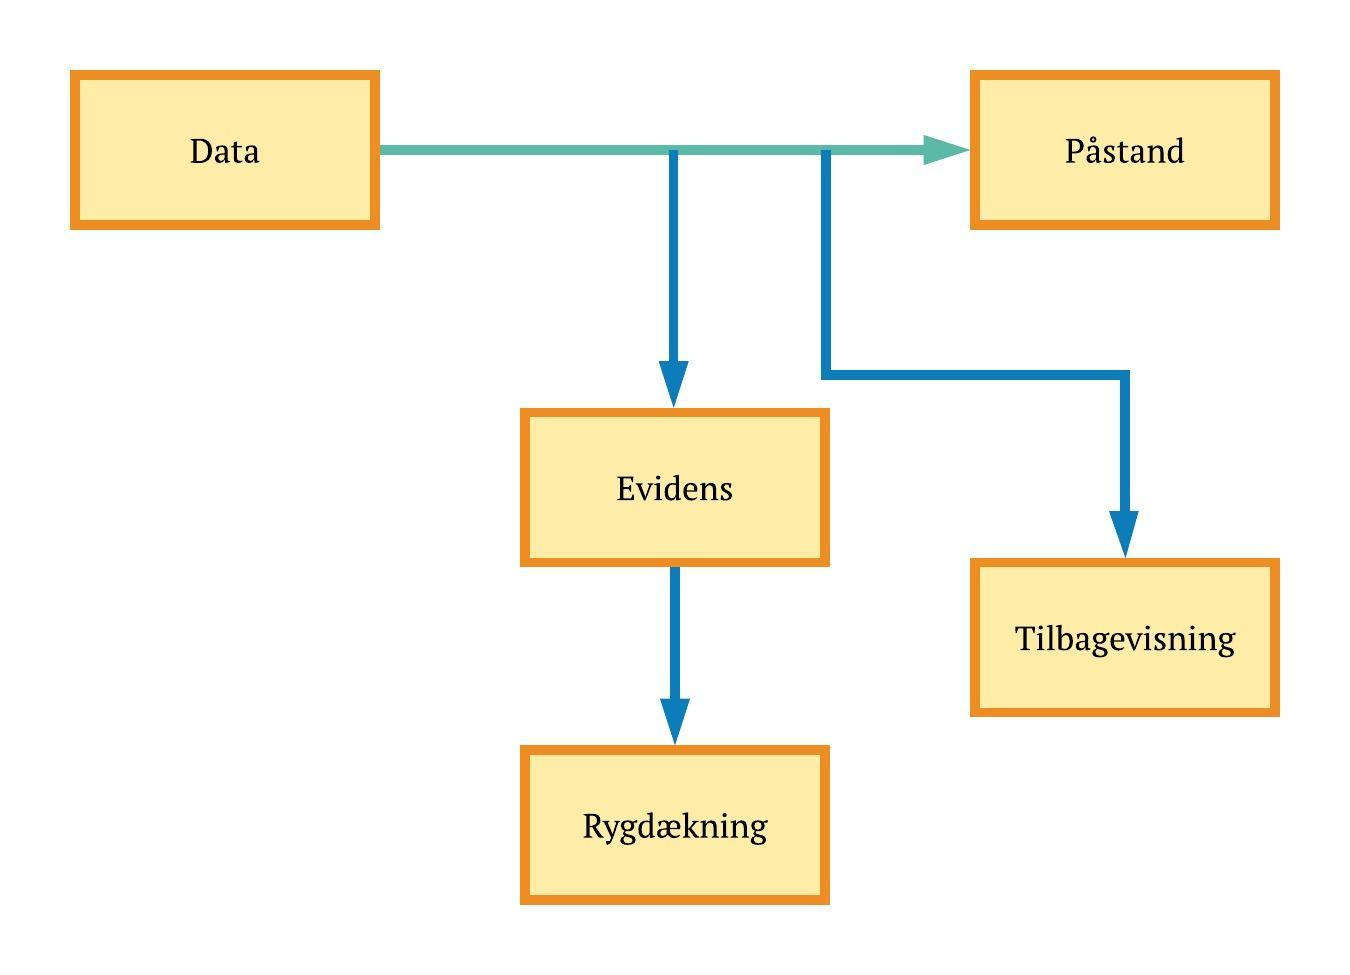
\includegraphics[width=.75\textwidth]{Figs/Toulmin}
	\caption[Toulmin's Argumentations Princip]{Skematisk tegning af Toulmins model for argumentation efter \citet{Toulmin1958}.}
	\label{fig:tou}
\end{figure}

I analysen af elevernes skriftlige arbejde undersøges det altså hvorvidt eleverne laver påstande på baggrund af deres data samt hvorvidt de har evidens og rygdækning for deres påstande. Hvis ikke og modellen tipper mod en tilbagevisning så betragtes det hvorledes eleverne kommer om ved at reflektere over hvad der så kan gøres for at forbedre udfaldet.

\subsubsection{Opsamling på Toulmin's argument pattern}
I forbindelse med dette projekt er TAP valgt for at sikre en ensartet måde at vurdere eleverens skriftlige arbejde efter et sæt af standard kriterier således at vi får et mål for om elevernes skriftlige kompetencer udvikeler sig gennem et undervisnings forløb med høj grad af \ib{}. 

\section{Litteratursøgning}
\label{sec:lit}

Processen med at udvælge primær litteratur til dette speciale er forløbet i henhold til følgende principper, som ligeledes er illustret på  figur\vref{fig:21a}. Jeg har valgt at dele denne process ind i 5 trin som er gennem løbet på følgende vis og gennem følgende kriterier. Først gennemførtes en søgning på Google scholar med følgende udsagn ``\emph{practical work AND science writing heuristic}''. Det er klart at der er behov for en grovere sortering med et udgangspunkt på 335\,000 hits. 

I trin to lavede jeg en sørning på \url{http://library.au.dk} med den samme søge tekst og med et ekstra kriterium nemlig at kilderne skulle være skrevet fra og med 1999. For at få nyere forskning tilgængelig dette reducerede antallet af hits til 21\,551. 
\begin{wrapfigure}{o}{0.5\textwidth}
	\centering
	\vspace{-20pt}
	\smartdiagram[descriptive diagram] {
		{Trin 1, 335\,000 hits via Søgning på Google Scholar},
		{Trin 2, 21\,551 hits via søgning på library.au.dk},
		{Trin 3, 15 hits opdaterede søge kriterier},
		{Trin 4, 10 hits screening af abstracts},
		{Trin 5, 8 hits fra sortering af fejl screenede kilder},
	}\vspace{0pt}
	\caption[Litteratursøgningsprocessen]{Grafisk fremstilling af litteratursøgningsprocessen}
	\label{fig:21a}
	\vspace{-20pt}
\end{wrapfigure}
Det næste skridt var blev at opdatere tidskriteriet til at være artikler som er skrevet efter 2005. Dette snævrede feltet betydeligt ind og ved at kræve at litteraturen skulle handle om skriftlighed og praktiskarbejde blev i fagene fysik og kemi blev feltet reduceret betydeligt til blot 15 hits i skridt tre.

Herefter blev alle 15 abstracts screenet med henblik på at afdække om der var eventuelt dobbeltgængere i mellem dem, samt abstracts som ikke var hjemmehørende i dette projekt. Her blev også skeelet til hvilken skoleform der var tale om. Er det gymnasialt niveau eller er der tale om undervisning på universitets niveau. Dette reducerede yderligere omfanget af kilder til 10.

Efter gennemlæsning af litteraturen stod det klart at der var dele af litteraturen som ikke var anvendelig i forbindelse med denne opgave dette viste sig at gælde for to af de tilbageværende artikler de blev derfor kasseret. Dermed baseres nedenstående litteratur review sig på 8 artiker som er fundet på baggrund af den ovenfor beskrevne litteratursøgningsprocess. I det følgende afsnit \vref{sec:2.2} ser vi på hvilke temaer der kan uddrages af artiklerne, forud for det egentlige review af artikelerne i afsnit \vref{sec:2.4}. 


\section{Temaer i litteraturen}
\label{sec:tem}

Betrægtes de artiker som blev fundet på basis af litteratursøgningsprocessen ovenfor så er der en tydelig række af fællesnævnere som går igen uafhængigt af om artiklen handler om begrebet \emph{Writing to Learn} hvor man arbejder med at øge eleverne faglige udbytte gennem det skriftlige arbejde. eller der er tale om artikler med særligt fokus på \emph{science writing heuristic} som fokus, så er der i litteraturen konsensus for at man ikke bør sætte eleverne til at skrive rapport i en mere klassisk forstand da dette på ingen måde fremme elevernes læring. \citep{Akkus2007, Atasoy2013, Burke2005, Keys1999}. Det er også i denne kontekst at \citet{Hodson2008} kommer til udtryk med sin tese om \emph{'``... at det kan være direkte kontra produktivt at lave praktisk arbejde med eleverne''}. \citet{Krogh2016,Dolin2014} peger på at en løsning på denne udfordring kunne være at lade eleverne arbejde mere undersøgelsesbaseret i naturfagene og ikke blot i fysik faget. 

En del af løsningen på udfordringen præsenteres af \citep{Keys1999, Burke2005} i form af en ny tilgang til skriftligheden i naturfagene. Her peges der i retning af en skriftlig struktur som er mere undersøgende i sin natur. Humlen i alt dette er at vi skal gentænke den måde hvorpå vi strukturerer det skriftlige forløb for eleverne. \citet{Burke2005} foreslår en ny tilgang til den skriftlige skabelon som vi har anvendt i mange år i det danske gymnasium, denne nye skabelon er bygget ovenpå SWH som udarbejdet af \citep{Keys1999}, og forskellen mellem de to tilgange er givet i tabel \vref{tbl:2.1}.

\begin{table}
	\centering
	\caption[Rapport skabeloner]{Her ses forskellen mellem strukturen i en klassisk fysik rapport og en mere undersøgelsesbaseret tilgang til rapporten jf. IBSE og SWH. Tabellen er hentet fra hhv. 
	\citet{Burke2005, Keys1999}.}
	\label{tbl:2.1}
	\begin{tabular}{@{ } l l @{ }}
		\toprule[2.5pt]
			\multicolumn{2}{c}{Rapport skabelon}\\
			\multicolumn{1}{c}{Klassisk} & \multicolumn{1}{c}{\ib{}/SWH}\\
		\midrule[1.25pt]
			Titel				&	Titel\\
			Introduktion			&	Undersøgelsesspørgsmål\\
			Formål			& 	Tests/Eksperimenter\\
			Teori \& fremgangsmåde		&	Observationer\\
			Data \& observationer	&	Påstande baseret på data\\
			Databehandling		&	Evidens for påstande\\
			Diskussion			&	Refleksioner\\
			Konklusion			&	Refleksion over egen læring\\
		\bottomrule[2.5pt]
	\end{tabular}
\end{table}

Største delen af de fundne artikler peger på en målbar effekt af indførelsen af SWH i undervisningen, givet at der arbejdes fokuseret med skriftliged i den daglige undervisning i et forløb med en varighed på 8 - 12 uger. Der er med andre ord tale om en signifikat påvirkning af elevernes læring og udvikling af deres skriftlige kompetence gennem en kortere periode. Kun artiklen af \citep{Miller2018} nævner ikke effekterne af SWH, hvilket skyldes at dette mere er et review af forskningsfeltet indenfor skriftlighed i den gymnasiale sektor. Hvis vi ser bort fra artiklen af \citep{Miller2018, Dolin2014, Krogh2016} arbejder forskerne bag undersøgelserne ud fra principperne i mixed-methods tilgangen til eksperimenterne. Desuden er størstedelen af artiklerne klart positivistiske i den forstand at der gennemføres en pre-test, efterfulgt af en intervension og hele forløbet afsluttes med en post-test. På denne måde får de en mere eller mindre validt mål for effekten af intervensionen blandt eleverne. Samtidig forholder de sig også til de kulturelle effekter i undervisning som også kan påvirke deres resultater, hvilket nok trækker dem i retning af mere post-positivistiske end blot positivistiske.


\section{Litteraturreview}
\label{sec:rev}

På de danske ungdomsuddannelser arbejder eleverene i høj grad eksperimentelt i de naturvidensjkabelige fag. Dette pratiske arbejde gennemføres i høj udstrækning efter vejledninger som kan karakteriseres som \emph{kogebogsvejledninger}. Med kogebogsvejledninger menes øvelsesvejledninger hvor alle dele af det pratiske arbejde er udførligt beskrevet for eleven i stil med opskrifterne i en kogebog, således at eleverne er klar over hvad de skal gøre samt hvordan de skal gøre det igennem hele øvelsen. Dermed bliver øvelsens formål at få eleverne til at reproducere allerede kendte resultater for at \emph{eftervise} allerede kendte sammenhænge fra teorien. Det store review af \citep{Miller2018} peger sammen med \citep{Hodson2008} på at udbyttet af denne mere traditionelle form for praktisk arbejde er relativt begrænset, eller i hvertfald begrænset til at indøve elementære laboratoriefærdigheder. \citep{Hodson2008} går skridtet videre og antyder at det kan være direkte spild af tid og ressourcer at lade eleverne gennemfører denne type af øvelser i laboratoriet.  I følge \citep{Hodson2008} er der en forskel mellem hvad eleverne reelt får ud af øvelserne  og det underviserne forventer at eleverne får ud af øvelserne. Dette baseres på at underviserne i studier giver udtryk for at de føler at eleverne motiveres ved at skulle foretage beregninger baseret på egne data. Denne påstand har man dog imidlertid ikke kunne påvise i undersøgelser, blandt eleverne. \citet{Krogh2016} skriver følgende opsummering,
\begin{quote}
``[\ldots]\emph{studierne viser derimod at eleverne ikke opfatter øvelserne som voldsomt spændnde - men de giver variation og opfattes som mindre kedelige end den daglige naturfagsundervisning}[\ldots]''
\end{quote}
Ungdomsuddannelsernes fokus har derfor gennem de senere år flyttet sig i retning af IBSE undervisning som den beskrives i hhv. \citep{Dolin2014, Krogh2016}. Med den stigende interesse for IBSE tilgangen til naturfagsundervisningen flyttes fokus fra reproduktions øvelser til øvelser hvor eleverne i højere grad skal drive øvlsen fremad. Herved kommer eleven i centrum for øvelsen og det bliver elevens undren over fænomener som bliver bestemmelnde for hvad eleverne undersøger i laboratoriet. Øvelsen flyttes altså fra ren \emph{reproduktion} over mod \emph{konstruktion} af viden som det også beskrives af \citep{Krogh2016}. Når man fundementalt ændre på den måde hvorpå man gennemfører øvelser får man brug for at kigge på den måde som eleverne afrapportere deres undersøgelser er den klassiske rapport, se tabel \vref{tbl:2.1} den bedste metode?  Her peger flere kilder \citep[m.fl.]{Burke2005, Erkol2010} på at eleverne skal anvende en ny type afrapportering nemlig SWH som blev introduceret af \citep{Keys1999}. Med SWH som tilgang til skriftligheden flyttes også rapportens fokus ligeledes fra reproduktion af viden til konstruktion af viden hos eleverne. \citet{Keys1999} skriver selv om ændringen 
\begin{quote}
``[\ldots]\emph{Postmodernister peger på at elever skal lære måder at udtrykke sig på som tillader dem at kritisere den status quo som findes i det videnskabelige dogmæne, hvorimod konstruktivister er af den opfattelse at eleverne skal lære udtryksformer som repræsentere konstruktionen af personlig og social udviklende meninger\, ~\ldots~ SWH-formen tilbyder netop en ramme for den videnskabelige skrive proces som i et vist omgang understøtter begge sunspunkter}[\ldots]''
\end{quote}
Sluttelig peger \citep{Keys1999} på at SWH-formen gennem refleksiv kognition og i samspil med andre elever og underviseren vil skabe en mere rodfæstet erkendelse unden for det videnskabelige dogmæne.  Flere studier \citep[m.fl.]{Akkus2007, Burke2005} har undersøgt hvordan det går med implementeringen af de nye tiltag med særligt fokus på IBSE. Studierne påviser at der en stor vilje til at ændre praksis blandt underviserne, men at de samme undervisere har svært ved at indfører disse nye undervisningsformer uden en grundig indføring og uden at have afprøvet formen på egen krop. Af \citep{Erkol2010} fremgår det at man ønsker at teste implementeringen af SWH blandt en gruppe af første års fysik studerende på et universitet i det østlige Tyrkiet.  Emnet hvori man introducerede de nye studerende for SWH var i fysik faget inden for mekanik, i artiklen finde de at der over en periode svarende til det første semester hvor hhv. test gruppen og kontrolgruppen kun introduceres til hvordan man implementerer laboratoriearbejde og hvordan dette afrapporteres, herefter blev de to grupper undervist efter forskellige fremgangsmåder. Her viste før og efter tests at der var en signifikant forskel mellem de studerendes forståelse af emnet mekanik. Endvidere skriver \citet{Erkol2010} at i tillæg peger 71.6 \% af de studerende på at udarbejdelsen af den traditionelle rapport var direkte kedelig (23.8 \% nogenlunde enig, 19.4 \% enig og 28.4 \% helt enig). De studerende i testgruppen peger på at SWH strategien øger deres læring og de finder at laboratoriearbejdet mere meningsfuldt. Endvidere peger 87.6 \% af testpersonerne på at SWH-rapport formatet er med til at udvikle deres problemløsningsevner. \citep{Erkol2010} slutter af med at pege på at lingende studier i andre naturfag har afstedkommet lignende eller identiske udfald, hvilket indikerer stor validitet, når man kan opnå sammenlignlige resultater på tværs af fag og emner med den samme grundlæggende metode. \citep{Atasoy2013} tager over hvor \citep{Erkol2010} slutter, her gennemfører man et studium inden for det fysik faglige område, med særligt fokus på begrebet Writing-to-Learn (WtL) en metode som også favnes af SWH. Motivationen for at gå i gang med dette projekt for \citep{Atasoy2013} er at der mangler studier på netop dette område. I modsætning til \citet{Erkol2010} som beskriver sine testpersoner som førsteårs studerende, beskriver \citet{Atasoy2013} sine testpersoner som bachelorstuderende, og hun har valgt at anvende emnet elektrostatik til sin undersøgelse. Testpersonerne følges her gennem en otte ugers periode, og konklusionen er at de studerende som anvender en WtL strategi i deres daglige arbejde opnår en højere konceptuel forståelse end de elever som ikke anvender en WtL-tilgang til det pratiske arbejde i laboratoriet. For at vi kan sige at dette er rammende for eleverne på de danske ungdomsuddannelser herunder STX bør man også undersøge elever som er på stadiet lige inden de skal på ungsomsuddannelserne. Derfor rettes blikket nu mod \citep{Kingir2013}. Her undersøger man en række 9. klasses elevers udbytte af at anvende SWH som et middel til at øge forståelsen af fænomenter inden for kemiens emne område. \citet{Kingir2013} finder på samme vist som \citet{Atasoy2013, Erkol2010} at elevernes konceptuelle forståelse af det faglige stof stiger over projekt perioden, samt at elevernes evne til at løse problemstillinger øges markant. Hvis SWH er sådan en god ide hvorfor er der så ikke flere som har valgt at skifte de traditionelle øvelser med dertilhørende rapport ud, med undersøgelsesbaserede øvelser med dertilhørende skriftligt arbejdes udfærdiget efter SWH modellen? Forklaringen skal i følge \citet{Burke2005,Keys1999,Krogh2016} vindes i det faktum at yngre undervisere faktisk gerne vil skifte men ikke nødvendigvis evner skiftet fra en undervisningsform til en anden på grund af en relativt begrænset værktøjskasse. I mens ældre undervisere i princippet har værktøjerne tila t foretage skiftet men mangler lysten til at skifte til den nye form. Derfor forbliver det en kamp for de få at sikre en bedre eksperimentel undervisning i naturfagene herunder også fysik.

